

Izmantojot \textit{SpikingJelly} ietvaru ar temporālu impulsu kodēšanu 4 laika soļos, apmācīti trīs konvolucionāli \Gls{snn} modeļi, lai novērtētu piedāvāto realizāciju dažādos tīkla mērogos. Pirmais ir kompakts divslāņu tīkls, kas apmācīts ar \textit{MNIST} datu kopu. Otrais un trešais ir dziļāki tīkli, kas apmācīti \textit{Caltech-101} attēlu klasifikācijas uzdevumam, izmantojot attiecīgi četrus un sešus konvolūcijas slāņus. Trīs tīklu arhitektūras ilustrētas \ref{fig:evaluation_networks}. attēlā.

Divslāņu \textit{MNIST} tīkls sastāv no konvolūcijas slāņiem ar 8 un 16 izejas kanāliem, izmantojot \(3\times3\) kodolus. Četrslāņu \textit{Caltech-101} tīkls sastāv no konvolūcijas slāņiem ar 8, 16, 32 un 64 izejas kanāliem, arī izmantojot \(3\times3\) kodolus. Sešslāņu \textit{Caltech-101} tīklam kanālu konfigurācija ir \(8, 16, 32, 32, 64, 64\) ar \(3\times3\) kodoliem. Starp izvēlētiem konvolūcijas slāņiem ievietoti apvienošanas slāņi ar \(2\times2\) logiem, lai samazinātu telpiskos izmērus.

Četrslāņu \textit{Caltech-101} tīkls apmācīts un novērtēts, izmantojot datu kopas pirmās piecas klases, savukārt sešslāņu
tīklam izmantotas pirmās desmit klases. Tas nodrošina divus arvien sarežģītākus klasifikācijas uzdevumus, vienlaikus
palielinot tīkla dziļumu. Šīs konfigurācijas ļauj novērtēt \Gls{fpga} realizācijas mērogojamību.

\begin{figure}[!t]
    \centering
    \begin{subfigure}{0.32\linewidth}
        \centering
        % 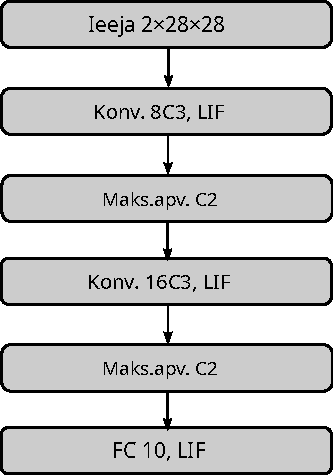
\includegraphics[width=\linewidth]{fig/lv/layer_structure_2.pdf}
        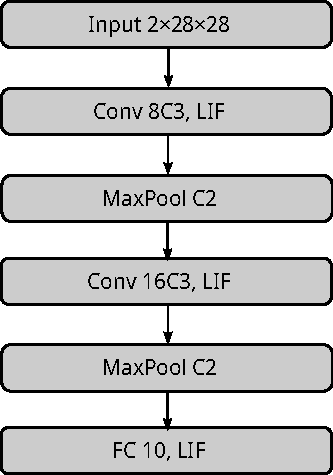
\includegraphics[width=\linewidth]{fig/layer_structure_2.pdf}
        \caption{MNIST, 2 slāņi.}
        \label{fig:layer_structure_2}
    \end{subfigure}
    \hfill
    \begin{subfigure}{0.32\linewidth}
        \centering
        % 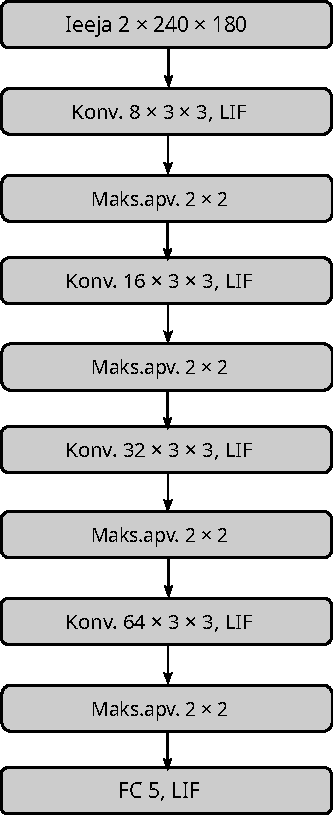
\includegraphics[width=\linewidth]{fig/lv/layer_structure_4.pdf}
        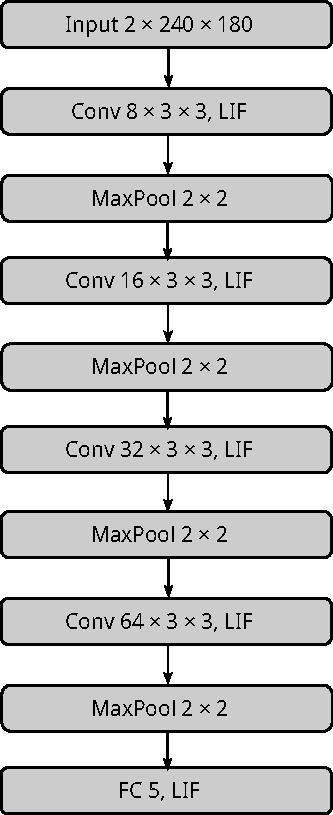
\includegraphics[width=\linewidth]{fig/layer_structure_4.pdf}
        \caption{Caltech-101, 4 slāņi.}
        \label{fig:layer_structure_4}
    \end{subfigure}
    \hfill
    \begin{subfigure}{0.32\linewidth}
        \centering
        % 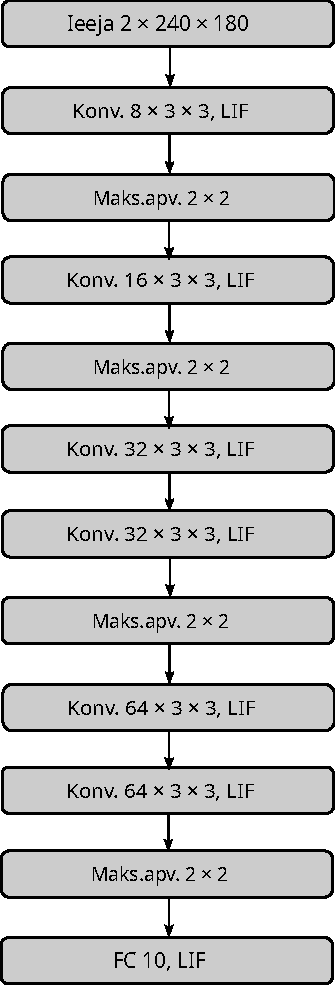
\includegraphics[width=\linewidth]{fig/lv/layer_structure_6.pdf}
        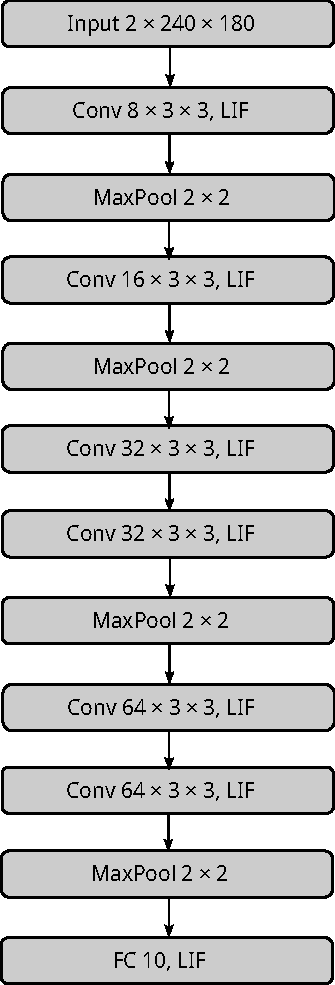
\includegraphics[width=\linewidth]{fig/layer_structure_6.pdf}
        \caption{Caltech-101, 6 slāņi.}
        \label{fig:layer_structure_6}
    \end{subfigure}
    \caption{Eksperimentālajā novērtējumā izmantotās SNN arhitektūras:
    (\subref{fig:layer_structure_2}) divslāņu MNIST tīkls,
    (\subref{fig:layer_structure_4}) četrslāņu Caltech-101 tīkls un
    (\subref{fig:layer_structure_6}) sešslāņu Caltech-101 tīkls.}
    \label{fig:evaluation_networks}
\end{figure}

Apmācības laikā pēc konvolūcijas slāņiem ievietoti pakešu normalizācijas slāņi, lai uzlabotu optimizāciju un apmācības stabilitāti. Inferences laikā pakešu normalizācija tiek apvienota ar konvolūcijas svariem un nobīdēm. Tādēļ pakešu normalizācijai nav nepieciešams atsevišķs aparatūras slānis un tā nav parādīta \ref{fig:evaluation_networks}. attēlā.

Svariem piemērota \Gls{ptq} ar dažādiem bitu platumiem, lai novērtētu tās ietekmi uz klasifikācijas veiktspēju. Kā parādīts
\ref{tab:quant_compare}. tabulā, abiem modeļiem F1 rādītājs samazinās tikai nedaudz līdz pat 4 bitu precizitātei, savukārt,
samazinot bitu platumu zem 4 bitiem, veiktspēja kļūst nestabila. F1 rādītāja atšķirības saglabājās 1~\% robežās attiecībā
pret 32 bitu atskaites vērtību. Samazinot sešslāņu tīkla svaru precizitāti līdz 2 bitiem, F1 rādītājs ievērojami samazinājās līdz
41,98~\%, norādot, ka jutība pret kvantēšanu ir atkarīga no tīkla dziļuma.

\begin{table}
\centering
\caption{Kvantēšanas ietekme uz SNN arhitektūru inferences F1 rādītāju}
\label{tab:quant_compare}
\begin{tabular}{@{}lccccc@{}}
\toprule
\textbf{Kvantēšana}       & \textbf{32 biti} & \textbf{16 biti} & \textbf{8 biti} & \textbf{4 biti} & \textbf{2 biti}    \\ \midrule
\multicolumn{6}{c}{28\texttimes 28-8C3-P2-16C3-P2} \\
\midrule
F1 rādītājs MNIST [\%]        & 96{,}78   & 96{,}80   & 96{,}81   & 96{,}79   & 90{,}10   \\
\midrule
\multicolumn{6}{c}{240\texttimes 180-8C3-P2-16C3-P2-32C3-P2-64C3-P2} \\
\midrule
F1 rādītājs Caltech-101 [\%]  & 88{,}87   & 88{,}67   & 89{,}07   & 89{,}32   & 87{,}19   \\
\midrule
\multicolumn{6}{c}{240\texttimes 180-8C3-P2-16C3-P2-32C3-32C3-P2-64C3-64C3-P2} \\
\midrule
F1 rādītājs Caltech-101 [\%]  & 87{,}99 & 87{,}37  & 86{,}85  &  88{,}10  & 41{,}98 \\
\bottomrule
\end{tabular}
\end{table}

Inferences latentuma salīdzināšanai kvantētie \Gls{snn} modeļi izpildīti \textit{NVIDIA GeForce RTX 5070 Ti}, \textit{NVIDIA Jetson AGX Orin} un \textit{Kintex UltraScale KU115-2} \Gls{fpga} platformās. Salīdzinājums ietvēra divslāņu \textit{MNIST} modeli un četrslāņu un sešslāņu \textit{Caltech-101} modeļus. \ref{tab:execution_time}. tabulā parādīti katrai platformai izmērītie apstrādes laiki, datu pārsūtīšanas laiki un kopējie inferences latentumi. \Gls{fpga} sasniedza attiecīgi \qty{1.10}{\milli\second}, \qty{2.43}{\milli\second} un \qty{2.81}{\milli\second} kopējo latentumu trim tīkliem. Salīdzinājumā ar \textit{Jetson AGX Orin} šie rezultāti parāda latentuma samazinājumu attiecīgi par \qty{2.30}{\milli\second}, \qty{2.35}{\milli\second} un \qty{3.60}{\milli\second}. \textit{RTX 5070 Ti} visiem trim tīkliem sasniedza mazāku kopējo latentumu nekā \Gls{fpga}, ar atšķirību attiecīgi \qty{0.30}{\milli\second}, \qty{1.28}{\milli\second} un \qty{1.66}{\milli\second}. Šie rezultāti demonstrē, ka piedāvātais \Gls{fpga} paātrinātājs nodrošina mazāku inferences latentumu nekā iegultā GPU platforma, lai gan augstas veiktspējas diskrētais GPU pārbaudītajiem tīkliem joprojām ir ātrāks.

\begin{table}[t]
\centering
\caption{Inferences latentums FPGA un GPU aparatūras platformām, izmantojot tīklus ar 2 un 4 konvolūcijas slāņiem
}
\label{tab:execution_time}
\begin{tabular}{lcccc}
\toprule
\textbf{Ierīce} & \textbf{Sinhr. uz} & \textbf{Apstrāde} & \textbf{Sinhr. no} & \textbf{Kopā} \\
 & \textbf{ierīci (ms)} & \textbf{(ms)} & \textbf{ierīces (ms)} & \textbf{(ms)} \\
\midrule
\multicolumn{5}{c}{28\texttimes 28-8C3-P2-16C3-P2} \\
\midrule
RTX5070 Ti & 0{,}05 & 0{,}70 & 0{,}05 & 0{,}80 \\
UltraScale KU115-2 & 0{,}08 & 0{,}95 & 0{,}08 & 1{,}10 \\
Jetson AGX Orin & 0{,}75 & 2{,}10 & 0{,}55 & 3{,}40 \\
\midrule
\multicolumn{5}{c}{240\texttimes 180-8C3-P2-16C3-P2-32C3-P2-64C3-P2} \\
\midrule
RTX5070 Ti & 0{,}06 & 1{,}00 & 0{,}06 & 1{,}12 \\
UltraScale KU115-2 & 0{,}09 & 2{,}25 & 0{,}09 & 2{,}43 \\
Jetson AGX Orin & 0{,}90 & 3{,}15 & 0{,}70 & 4{,}75 \\
\midrule
\multicolumn{5}{c}{240\texttimes 180-8C3-P2-16C3-P2-32C3-32C3-P2-64C3-64C3-P2} \\
\midrule
RTX5070 Ti & 0{,}07 & 1{,}02 & 0{,}06 & 1{,}15 \\
UltraScale KU115-2 & 0{,}09 & 2{,}64 & 0{,}08 & 2{,}81 \\
Jetson AGX Orin & 0{,}94 & 4{,}87 & 0{,}60 & 6{,}41 \\
\bottomrule
\end{tabular}
\end{table}

\ref{tab:sparsity}. tabulā piedāvātais paātrinātājs salīdzināts ar esošām uz \Gls{fpga} balstītām konvolucionālo \Gls{snn} realizācijām. Lai gan esošie darbi galvenokārt orientēti uz sekliem tīkliem un vienkāršākām datu kopām, piemēram, \textit{MNIST}, piedāvātais risinājums atbalsta dziļākas arhitektūras un augstākas izšķirtspējas datu kopas (piemēram, \textit{Caltech-101}), saglabājot konkurētspējīgu caurlaidību un mērenu resursu izmantojumu.

\begin{table}[t]
\centering
\footnotesize
\vspace{0.05in}
\caption{Uz FPGA balstītu CSNN realizāciju salīdzinājums iepriekšējos darbos un šajā darbā}
\label{tab:sparsity}
\begin{adjustbox}{max width=\textwidth}
  \begin{tabular}{@{}lp{1.7cm}p{1.7cm}p{1.7cm}p{1.7cm}p{1.6cm}p{1.6cm}p{1.6cm}@{}}
\toprule
\textbf{Darbs}       & \textbf{Sommer u.\,c.} \cite{sommer2022} & \textbf{Plagwitz u.\,c.} \cite{plagwitz2025} & \textbf{Zhang
    u.\,c. \cite{zhang2024b}} & \textbf{Zhang u.\,c. \cite{zhang2024b}} & \textbf{Šis darbs} & \textbf{Šis darbs} & \textbf{Šis darbs} \\ \midrule
Platforma            & XCZU7EV & XCZU9EG     & XC7Z020     & XC7Z020     & KU115-2 & KU115-2 & KU115-2 \\
Arhitektūra        & 3CL-1PL-1FC & 4CL-4PL-2FC & 2CL-2PL-1FC & 2CL-2PL & 2CL-2PL & 4CL-4PL & 6CL-6PL \\
Datu kopa             & MNIST & CIFAR-10    & MNIST       & Caltech-101 & MNIST   & Caltech-101 & Caltech-101 \\
\textbf{\(H \times W\)} & \(28 \times 28\) & \(32 \times 32\) & \(28 \times 28\) & \(240 \times 180\) & \(28 \times 28\) & \(240 \times 180\) & \(240 \times 180\) \\
\midrule
Resursi [LUTs]    & 19\,000 & 49\,930 & 628 & 1\,207 & 15\,627 & 41\,150 & 64\,687 \\
Resursi [FFs]     & 12\,000 & 28\,739 & -   & 1\,460 & 18\,671 & 59\,215 & 77\,122 \\
Resursi [BRAM]    & 2{,}1 Mib & 1{,}93 Mib & - & 1{,}25 Mib & 1{,}84 Mib  & 4{,}42 Mib & 5{,}07 Mib \\
Resursi [DSPs]    & 32     & 0      & -   & 0      & 0    & 0       & 0       \\
Kvantēšana [biti] & 8     & 4      & 2   & 2     & 8      & 8      & 8      \\
\bottomrule
\end{tabular}
\end{adjustbox}
\end{table}

\Gls{fpga} arhitektūras uzlaboto mērogojamību nodrošina hibrīda atmiņas organizācija, kurā sinaptiskie svari, dažādi \Gls{fifo}, \Gls{dma} buferi un starpsavienojumu buferi realizēti ar mikroshēmas iekšējo \Gls{bram}, savukārt membrānas potenciāli glabāti ārējā atmiņā un straumēti inferences laikā. Tādēļ tā paša tīkla realizācijai ar visiem membrānas potenciāliem mikroshēmā būtu nepieciešama papildu \Gls{bram} ietilpība.

Membrānas potenciālu atmiņas nepieciešamo apjomu tīklam ar \(L\) slāņiem aprēķina šādi:
\begin{equation}
  M_{\mathrm{memb}} = \sum_{l=1}^{L} C_l \times H_l \times W_l \times b_v,
\end{equation}
kur \(C_l\), \(H_l\) un \(W_l\) apzīmē attiecīgi membrānas potenciāla tenzora izejas kanālu skaitu, augstumu un platumu slānī
\(l\), un \(b_v=8\) biti ir šajā realizācijā izmantotā membrānas potenciāla precizitāte. Iegūtās glabāšanas prasības
novērtētajām tīklu konfigurācijām apkopotas \ref{tab:mp_resources}. tabulā.

Redzams, ka salīdzinājumā ar divslāņu \textit{MNIST} modeli četrslāņu un sešslāņu modeļi patērē ievērojami vairāk atmiņas, jo membrānas potenciālu apjoms pieaug līdz ar telpiskajiem izmēriem un dziļumu. Salīdzinājumā ar četrslāņu \textit{Caltech-101} tīklu sešslāņu konfigurācijai nepieciešams aptuveni par 19,9~\% vairāk membrānas potenciālu glabāšanas vietas.

\begin{table}[t]
\centering
\caption{Mikroshēmas iekšējās atmiņas prasības pilnībā iekšējai glabāšanai (svari un membrānas potenciāli iekšējā BRAM) un hibrīdai glabāšanai (membrānas potenciāli ārējā SDRAM un svari iekšējā BRAM)}
\label{tab:mp_resources}
\begin{tabular}{lcccc}
\toprule
  \textbf{Arhitektūra} & \textbf{Ārējā} & \textbf{Visa mikroshēmā} & \textbf{Samazinājums}\\
\midrule
  28\texttimes 28-2CL-2PL   & 73{,}50Kib & 1{,}91Mib  & 3{,}8~\% \\
  240\texttimes 180-4CL-4PL & 4{,}93Mib  & 9{,}35Mib  & 52{,}8~\% \\
  240\texttimes 180-6CL-6PL & 5{,}91Mib  & 10{,}98Mib & 53{,}9~\% \\
\bottomrule
\end{tabular}
\end{table}

„Hibrīda” realizācijas \Gls{bram} izmantojums, kas norādīts \ref{tab:sparsity}. tabulā, jau ietver svariem, dažādiem
\Gls{fifo} buferiem un starpsavienojumu buferēšanai piešķirto mikroshēmas iekšējo atmiņu, bet neietver membrānas potenciālu
glabāšanu. Lai novērtētu papildu \Gls{bram} ietilpību teorētiskai pilnībā mikroshēmā izvietotai realizācijai, membrānas
potenciālu atmiņu var pieskaitīt nepieciešamajai svaru atmiņai. Tādējādi idealizēto \Gls{bram} daudzumu pilnībā mikroshēmā
izvietotai alternatīvai var izteikt kā
\begin{equation}
  M_{\mathrm{all\mbox{-}on\mbox{-}chip}}
  \approx M_{\mathrm{hybrid}} + M_{\mathrm{memb}},
\end{equation}
kur \(M_{\mathrm{hybrid}}\) apzīmē esošās hibrīda realizācijas aizņemto \Gls{bram} ietilpību (\ref{tab:sparsity}. tabula).
Relatīvo mikroshēmas iekšējās atmiņas nepieciešamo daudzuma samazinājumu, kas panākts, membrānas potenciālus glabājot ārēji, aprēķina šādi:
\begin{equation}
  R =
  \frac{M_{\mathrm{all\mbox{-}on\mbox{-}chip}} - M_{\mathrm{hybrid}}}
       {M_{\mathrm{all\mbox{-}on\mbox{-}chip}}}
  \times 100~\%.
\end{equation}
Kā parādīts \ref{tab:mp_resources}. tabulā, hibrīda atmiņas arhitektūra samazina teorētiskās mikroshēmas iekšējās atmiņas
prasības attiecīgi par 52,8~\% un 53,9~\% četrslāņu un sešslāņu \textit{Caltech-101} tīkliem. Redzams arī, ka hibrīda atmiņas
arhitektūras ieguvums ir atkarīgs no tīkla arhitektūras un membrānas potenciālu glabāšanas relatīvā ieguldījuma kopējā
iekšējā atmiņā. Divslāņu \textit{MNIST} tīklam membrānas potenciālu ārēja glabāšana samazina iekšējo atmiņu tikai par 3,8~\%,
jo membrānas potenciālu glabāšana veido samērā mazu daļu no kopējā atmiņas apjoma, savukārt četrslāņu un sešslāņu
arhitektūrām ir būtiski lielākas starpposmu pazīmju kartes un ar tām saistītā membrānas potenciālu atmiņa. Tas norāda, ka
mazāku pazīmju karšu gadījumā dominē citas atmiņas sastāvdaļas un membrānas potenciālu vērtības varētu glabāt pilnībā
mikroshēmā.

\ref{tab:power_usage}. tabulā parādīts vienas inferences enerģijas patēriņš četrslāņu \textit{Caltech-101} \Gls{snn} un
\Gls{ann} realizācijām. \Gls{snn} demonstrē būtiski mazāku enerģiju nekā \Gls{ann} pat vairākiem laika soļiem, galvenokārt
pateicoties retiem impulsu aprēķiniem un svaru glabāšanai mikroshēmas iekšējā BRAM. Tomēr stāvokļu atmiņas enerģija veido ievērojamu daļu no kopējās \Gls{snn} jaudas. Lai gan sinaptisko operāciju skaits \(N_{SynOp}\) ir daudz lielāks nekā neironu skaits \(N_{Neurons}\), atmiņas piekļuves enerģija saglabājas augsta ārpusmikroshēmas piekļuves lielo izmaksu dēļ, t.\,i., \(E_{SDRAM} >> E_{BRAM}\). Ieejas gadījums \(1 \times 2\) ir energoefektīvākais, aptuveni atbilstot \Gls{ttfs} konfigurācijai, kur membrānas potenciāli tiek atjaunināti tikai līdz pirmā impulsa rašanās brīdim.

Tomēr \Gls{ann} enerģijā dominē DRAM piekļuves svariem un aktivācijām, un int8 kvantēšana dod tikai nelielu ietaupījumu,
uzsverot \Gls{snn} impulsu retuma priekšrocības.

Lai gan analītiskais novērtējums nodrošina algoritmisko enerģijas priekšrocību atskaites vērtību, papildu tiek norādīts
\textit{Xilinx Power Analyzer} ziņotais patēriņš, ar kuru saskaņā kopējais dinamiskais jaudas patēriņš mikroshēmā ir 0,45~W. Atšķirība starp
izmērīto kopējo jaudu un analītisko novērtējumu tiek skaidrota ar kopējo mikroshēmas jaudu, tostarp takts signāla sadales
koku un PCIe DMA infrastruktūru. Neraugoties uz to, kopējā jauda saglabājas būtiski mazāka nekā augstas veiktspējas GPU
risinājumiem.

\begin{table}[h!]
\centering
\caption{Vienas inferences enerģijas patēriņš četrslāņu Caltech-101 SNN un ANN modeļiem, sadalot kopējo enerģiju sinaptisko operāciju un membrānas stāvokļu ieguldījumos}
\label{tab:power_usage}
\begin{tabular}{@{}lccccc@{}}
\toprule
\textbf{Modelis} & \textbf{\(T\times D\)} & \textbf{Kopējā enerģija (\unit{\micro\joule})} & \textbf{Sin./mem. enerģija (\unit{\micro\joule})}  \\ \midrule
SNN [int8]  & \(1 \times 2\)   & 120{,}201   & 64{,}290  / 55{,}910   \\
SNN [int8]  & \(4 \times 2\)   & 480{,}805   & 257{,}163 / 223{,}641  \\
ANN [int8]  & \(1 \times 1\)   & 414{,}719   &  -  \\
ANN [fl32]  & \(1 \times 1\)   & 466{,}624   &  -  \\
\bottomrule
\end{tabular}
\end{table}

Papildus jaudas mērījumi veikti tieši \textit{Alpha Data ADM-PCIE-8K5} paātrinātāja kartē inferences laikā. Kartē ir
sprieguma un strāvas sensori, kuru nolasījumi iegūti ar mikrokontrollera lietojumrīku. Jaudas rādījumi 12~V barošanas ķēdē
nepārtraukti reģistrēti 10\,000 paraugu intervālā dīkstāvē un aktīvas inferences laikā četrslāņu \textit{Caltech-101} tīklam
($T\times D = 4\times 2$). \ref{tab:measured_power_stats}. tabulā norādītās jaudas vērtības ir reģistrēto paraugu vidējā
vērtība un standartnovirze.

Dīkstāvē kartes vidējais kopējais jaudas patēriņš bija $15{,}771 \pm 0{,}069\,\text{W}$. Inferences laikā vidējais jaudas patēriņš pieauga līdz $15{,}862 \pm 0{,}070\,\text{W}$. Lai atšķirtu inferences papildu jaudu no platformas dīkstāves jaudas, izmērīto dinamisko jaudas patēriņu definē šādi:
\begin{equation}
    P_{\mathrm{dyn}} =
    P_{\mathrm{inference}} - P_{\mathrm{idle}}.
\end{equation}
Papildu enerģija vienai inferencei novērtēta, kopējās platformas jaudas vietā izmantojot \(P_{\mathrm{dyn}}\). Starpība starp izmērītajām vidējām vērtībām norāda uz aptuveni $91\,\text{mW}$ paātrinātāja jaudas patēriņu. Testa laikā vidējais vienas inferences ilgums bija \qty{2.4}{\milli\second}, un vienas inferences enerģija bija 218,4~$\mu$J. Nelielais dinamiskās jaudas pieaugums apstiprina, ka kopējā patēriņā dominē PCIe kartes statiskā jauda, savukārt uz notikumiem balstītais \Gls{snn} kodols veic energoefektīvus aprēķinus.

\begin{table}[htbp]
\centering
\caption{ADM-PCIE-8K5 FPGA paātrinātāja kartes jaudas un enerģijas mērījumi dīkstāvē un aktīvas inferences laikā ($T\times D = 4\times 2$, četrslāņu Caltech-101 modelis, 10\,000 paraugu)}
\label{tab:measured_power_stats}
\begin{tabular}{l r r}
\toprule
\textbf{Metrika} & \textbf{Dīkstāve} & \textbf{Inference} \\
\midrule
Vidējā jauda & 15{,}771 $\pm$ 0{,}069 W & 15{,}862 $\pm$ 0{,}070 W \\
Min./maks. jauda & 15{,}572 / 15{,}975 W & 15{,}722 / 16{,}055 W \\
Inferences jauda & -- & 91 mW \\
Vidējais inferences laiks & -- & \qty{2.4}{\milli\second} \\
Vienas inferences enerģija & -- &  218{,}4 $\mu$J \\
\bottomrule
\end{tabular}
\end{table}


